\section{Method}
\label{sec:method}

\begin{figure}[ht]
\centering
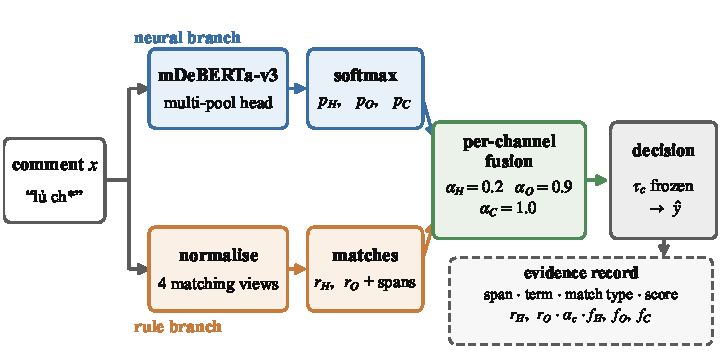
\includegraphics[width=\textwidth]{figures/architecture.pdf}
\caption{The hybrid. A comment enters two independent branches. The neural branch
produces class probabilities; the rule branch produces per-label lexical scores and
the spans that produced them. Fusion mixes each channel with its own weight
$\alpha_c$, and frozen per-channel thresholds turn the three scores into a label.
The evidence record is emitted with the decision and makes the lexical part of the
decision inspectable. Weights and thresholds shown are the values selected on
validation for the focused backbone.}
\label{fig:architecture}
\end{figure}

The hybrid has three parts: a rule engine that produces lexical scores and spans, a
transformer that produces class probabilities, and a fusion layer that combines them
channel by channel (Fig.~\ref{fig:architecture}). The branches share no parameters,
which allows the rule branch to be audited on its own.

\subsection{The lexical rule engine}
\label{sec:rule-engine}

\paragraph{Normalisation and views.}
The comment is Unicode-normalised to NFC, invisible characters are removed,
whitespace is collapsed, character runs are shortened to at most three, and the text
is lower-cased while keeping Vietnamese diacritics. Normalisation returns an
\emph{offset map} to the raw comment, so a match on a cleaned view is always reported
as a span of the original text. Auxiliary views handle the writing tricks that matter:
accent-less, leet, repeat-collapsed, and a compact view with separators removed
(\texttt{n g u}). The matcher records, for every hit, the dictionary term, label, view,
raw span and a \emph{match type} (\emph{exact}, \emph{accentless\_alias}, \emph{leet},
\emph{repeat\_collapsed}, \emph{separator\_inserted}, \emph{obfuscated\_combined} or
\emph{fuzzy}).

\paragraph{Scoring.}
Every match $i$ receives
\begin{equation}
s_i \;=\; \sigma_{\ell(i)} \cdot c_i \cdot m_i \cdot \kappa_i ,
\label{eq:match}
\end{equation}
where $\sigma_{\ell(i)}$ is the severity of the matched label ($0.95$ for
\hate{}, $0.60$ for \off{} after tuning), $c_i$ the entry confidence from the
training split, $m_i$ the match-type factor and $\kappa_i$ a context factor for
quotation, negation and context-required terms. Matches of one label are
de-duplicated and aggregated with a saturating sum over at most $K=10$ matches:
\begin{equation}
r_\ell \;=\; 1-\prod_{i\in T_\ell}\left(1-s_i\right).
\label{eq:aggregate}
\end{equation}
For fusion they become a three-channel pseudo-probability
\begin{equation}
\tilde{\mathbf r} \;=\; \frac{1}{1+\min(r_H,r_O)}
\begin{bmatrix} r_H \\ r_O \\ 1-\max(r_H,r_O) \end{bmatrix},
\label{eq:pseudo}
\end{equation}
which preserves the ordering of the two toxic channels while placing \clean{} on
the same scale. When the rule is silent, $\tilde{\mathbf r}=(0,0,1)$: no evidence
is treated as maximal cleanliness evidence, the assumption that
Sect.~\ref{sec:analysis} tests.

\paragraph{Tuning.}
Scoring weights are tuned on validation by greedy coordinate descent, with
thresholds re-optimised for every candidate; test is never loaded. The search made
the engine more aggressive: severity \hate{} rose to $0.95$, the accentless-alias
factor was driven to $0.0$, the repeat-collapsed factor to $0.4$, the
combined-obfuscation factor to $0.3$, and the negation and context-required
factors to $1.0$. Validation preferred \emph{more} matches over \emph{cautious} ones:
the engine is a narrow, high-threshold detector, not a comprehensive obfuscation
detector.

\subsection{The neural branch}
\label{sec:neural}

We fine-tune \texttt{microsoft/mdeberta-v3-base}
\cite{he2023debertav3,liu2024mdeberta}. The focused backbone
(\model{sensitiveai-vi-custom}) uses a multi-pool head: the final hidden states are
pooled with the \texttt{[CLS]} token, mean pooling and max pooling, the three views
are concatenated, projected to a 512-dimensional bottleneck with dropout $0.1$, and
mapped to three logits. Training uses cross-entropy, AdamW
\cite{loshchilov2019adamw}, a linear schedule with $10\%$ warm-up, learning rate
$3\times10^{-5}$, effective batch size 32, maximum length 256 and at most 30 epochs,
with early stopping on validation macro-F1; the best checkpoint is frozen before
test. Three further backbones use the same encoder with different recipes: a
standard-head baseline, a two-stage model with discriminative learning rates and
focal loss \cite{lin2017focal}, and a three-stage curriculum
\cite{bengio2009curriculum} with manual class weights.

\subsection{Fusion and decision}
\label{sec:fusion}

Let $p_c$ be the transformer probability for class $c$ and $\tilde r_c$ the
renormalised rule score. Per-channel fusion is
\begin{equation}
f_c \;=\; \alpha_c\,p_c \;+\; (1-\alpha_c)\,\tilde r_c,
\qquad c\in\{\hate{},\off{},\clean{}\}.
\label{eq:fusion}
\end{equation}
A single global $\alpha$ is the special case $\alpha_H=\alpha_O=\alpha_C$. A class
is \emph{accepted} when $f_c\ge\tau_c$; the accepted class with the highest $f_c$
wins, and if none is accepted the decision falls back to $\arg\max_c f_c$.

We compare four families: global $\alpha$ with argmax, global $\alpha$ with
thresholds, a multinomial logistic meta-classifier over the six AI and rule scores,
and per-channel $\alpha$ with thresholds. All tunable quantities are selected on
validation and frozen before the single test pass. The per-channel variant is
primary because the classes have different rule behaviour: the rule channel is
precise on \hate{}, weak on \off{} and uninformative on \clean{}, so one $\alpha$
forces a bad compromise. Validation discovers the asymmetry: $\alpha_H=0.2$,
$\alpha_O=0.9$, $\alpha_C=1.0$, with
$\tau_H=0.14$, $\tau_O=0.66$, $\tau_C=0.60$. The \hate{} channel is 80\% lexical,
\off{} 90\% neural and \clean{} purely neural; the interaction between
$\alpha_H$ and $\tau_H$ drives Sect.~\ref{sec:analysis}.

\subsection{Evidence record and protocol}
\label{sec:evidence}

For every comment the system emits, with the label, an evidence record: matched
spans in the raw text, dictionary term and label of each span, matching view and
match type, per-match score, aggregated rule scores, per-channel weights and the
three fused scores. Given the record and the transformer probabilities, a reviewer
can recompute the decision exactly, which is what we mean by \emph{faithful by
construction} for the lexical channel; the neural contribution remains a black box,
and we do not claim otherwise. Every tunable quantity is frozen before the single test
pass, and the error analysis is descriptive and performed after it.
